%% The first command in your LaTeX source must be the \documentclass command.
\documentclass[acmtog]{acmart}
\usepackage[english,ngerman]{babel}
\usepackage[utf8]{inputenc} 
\usepackage{csquotes}

%% \BibTeX command to typeset BibTeX logo in the docs
\AtBeginDocument{%
  \providecommand\BibTeX{{%
    \normalfont B\kern-0.5em{\scshape i\kern-0.25em b}\kern-0.8em\TeX}}}
    
\copyrightyear{2024}
\acmYear{2024}
\citestyle{acmauthoryear}

\usepackage[figurename=Fig.]{caption}
\usepackage{csquotes}
\setcopyright{none}
\makeatletter
\renewcommand{\fnum@figure}{Abb. \thefigure}
\makeatother
\addto\captionsngerman{\renewcommand{\figurename}{Abb.}}
\settopmatter{printacmref=false} % Removes citation information below abstract
\renewcommand\footnotetextcopyrightpermission[1]{} % removes footnote with conference information in first column

%%
%% end of the preamble, start of the body of the document source.
\begin{document}

%%
%% The "title" command has an optional parameter,
%% allowing the author to define a "short title" to be used in page headers.
\title{Enterprise Architektur-Muster}

%%
%% The "author" command and its associated commands are used to define
%% the authors and their affiliations.
%% Of note is the shared affiliation of the first two authors, and the
%% "authornote" and "authornotemark" commands
%% used to denote shared contribution to the research.
\author{Julian Bruder}
\authornote{Alle Studierenden trugen zu gleichen Teilen zu dieser Arbeit bei.}
\author{Abdellah Filali}
\authornotemark[1]
\author{Luca Franke}
\authornotemark[1]
\affiliation{%
  \institution{Hochschule für Technik, Wirtschaft und Kultur Leipzig (HTWK Leipzig)}
  \streetaddress{Karl-Liebknecht-Str. 132}
  \city{Leipzig}
  %\state{Ohio}
  \country{Deutschland}
  \postcode{04277}
}
%%
%% By default, the full list of authors will be used in the page
%% headers. Often, this list is too long, and will overlap
%% other information printed in the page headers. This command allows
%% the author to define a more concise list
%% of authors' names for this purpose.
\renewcommand{\shortauthors}{Bruder, Filali, Franke}

%%
%% The abstract is a short summary of the work to be presented in the
%% article.
\begin{abstract}
Blah \ldots
\end{abstract}

\maketitle

\section{Einleitung}
% (Beschreibung von Kontext, Problemen, Anforderungen und Zielen)
Blah \ldots

\section{Grundlagen von Enterprise-Architekturen}
Blah \ldots

\section{Klassische Enterprise-Architekturen}
\subsection{Monolithic Architecture}
Der Begriff \textit{Monolith}, abgeleitet aus dem Altgriechischen und mit der Bedeutung
\textit{einheitlicher Stein}, wird in der Softwarearchitektur verwendet, um ein Designmuster
zu beschreiben, bei dem die gesamte Funktionalität einer Anwendung in einem einzigen,
zusammenhängenden System integriert ist.
In dieser Architektur übernimmt ein einzelner Prozess die Ausführung der gesamten Anwendung \cite[1]{mono}.

Anwendungen, die diesem Architekturansatz folgen, bestehen aus eng miteinander verknüpften
Komponenten, die wechselseitig voneinander abhängen.
Diese Komponenten können weder unabhängig betrieben noch, in bestimmten Fällen,
isoliert kompiliert werden \cite[485]{mono3}.

\begin{figure}[h!]
    \centering
    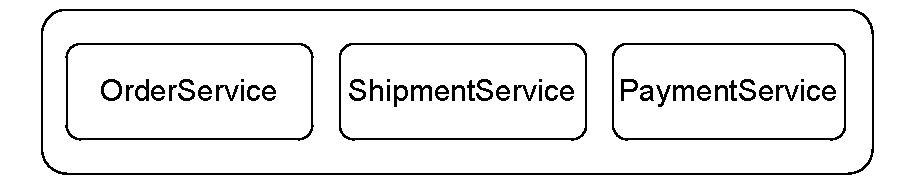
\includegraphics[width=0.4\textwidth]{images/mono/mono.pdf}
    \caption{Monolith Architektur}
    \label{fig:mono}
\end{figure}

Diese Architektur bietet insbesondere für kleinere Anwendungen mehrere Vorteile,
wie etwa eine vereinfachte Testbarkeit, Logging, Deployment und Debugging. Ein
weiterer Vorteil besteht darin, dass keine separate Datenbanksynchronisation
erforderlich ist, da sämtliche Daten in einer einzigen Datenbank gespeichert
werden \cite[2]{mono4}.

Betrachten wir das E-Commerce-Beispiel.
Dafür definieren wir drei Klassen:
\begin{itemize}
    \item \texttt{OrderService}: Klasse, die die Bestellungen verwaltet
    \item \texttt{PaymentService}: Klasse, die die Zahlungen abwickelt
    \item \texttt{ShipmentService}: Klasse, die die Lieferungen initiiert
\end{itemize}

Die Kommunikation zwischen den Klassen erfolgt über Methodenaufrufe. In diesem
Zusammenhang stellt die Klasse \texttt{OrderService} die zentrale Komponente dar,
die die Methoden anderer Klassen nutzt, um den Bestellprozess zu steuern. Ein
wesentlicher Vorteil dieses Ansatzes liegt in der einfachen Kommunikation
zwischen den Komponenten.
Durch den direkten Einsatz von Methodenaufrufen
wird die Komplexität verringert, die typischerweise mit der Interaktion zwischen
verschiedenen verteilte Systemen verbunden ist.
Die vollständige Implementierung des E-Commerce-Beispiels ist bei GitHub \footnote{https://github.com/Beleg-6-EAP/demo-monolith-ecommerce} zu finden.

Mit dem Wachstum und der zunehmenden Komplexität der Code-Basis treten jedoch
einige Nachteile auf.
Änderungen an einer Komponente können unerwartete kaskadierende
Fehler auslösen, was die Weiterentwicklung in kleinen, autonomen Teams erschwert
und verlangsamt.

Ein weiterer Nachteil ergibt sich aus der engen Kopplung zwischen den Komponenten,
die durch direkte Methodenaufrufe entsteht.
Änderungen an der Implementierung oder
der Signatur einer Methode können in der Folge die gesamte Anwendung beeinflussen.

Zudem wird die Wiederverwendung von Funktionalitäten erschwert, da die Komponenten
stark miteinander verknüpft sind.
Dies führt zu einer Duplizierung von Code, was die Kosten für Änderungen erhöht,
da diese an mehreren Stellen vorgenommen werden müssen.

Die daraus resultierende Komplexität und die erschwerte Wartung führen zu längeren
Iterationen.
Da das Deployment nur als Ganzes erfolgen kann, und die Iterationen
sich verlängern, kommt es zu seltenen Auslieferungen neuer Features.

Ein weiteres Problem liegt in der erschwerten horizontalen Skalierung, da die Anwendung
nur als Ganzes skaliert werden kann.
Dies stellt eine Herausforderung dar, da bei wachsenden
Anforderungen die gesamte Anwendung skaliert werden muss, anstatt einzelne Komponenten unabhängig
voneinander zu skalieren.

Insgesamt ist die monolithische Architektur eine geeignete Lösung für
kleinere Anwendungen, jedoch weniger geeignet für größere Systeme, da sie die Agilität und
Flexibilität erheblich einschränken kann.

\subsection{Modular Monolith}
Das Hauptproblem der zuvor beschriebenen Architektur liegt in der engen Kopplung der Komponenten,
was zu einer erhöhten Komplexität und begrenzten Flexibilität führt. Die Modular
Monolithic Architecture stellt eine Weiterentwicklung der Monolithic Architecture dar,
indem sie die Vorteile des monolithischen Ansatzes bewahrt und gleichzeitig die Nachteile
der engen Kopplung verringert.

In diesem Architekturmodell wird die Code-Basis in mehrere Module unterteilt, die jeweils
eine spezifische Teilfunktionalität der Anwendung implementieren.\cite[11]{modular-mono2}.

Die Modularisierung trägt zudem zur Reduzierung der Komplexität bei und ermöglicht eine bessere
Organisation der Code-Basis, was sich positiv auf die Wartbarkeit der Anwendung auswirkt \cite[23 - 24]{modular-mono4}.

\begin{figure}[h!]
    \centering
    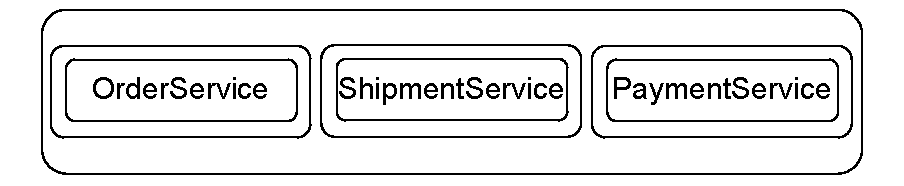
\includegraphics[width=0.4\textwidth]{images/mono/mono-example.pdf}
    \caption{Modular Monolith Architektur}
    \label{fig:modular-mono}
\end{figure}

Betrachten wir erneut das E-Commerce-Beispiel.
Diesmal wird die Anwendung in drei Hauptmodule aufgeteilt (Siehe Abb. ~\ref{fig:modular-mono}):
\begin{itemize}
    \item \texttt{order}: Modul, das für die Verwaltung der Bestellungen verantwortlich ist
    \item \texttt{payment}: Modul, das für die Abwicklung der Zahlungen verantwortlich ist
    \item \texttt{shipment}: Modul, das für die Initiierung der Lieferungen verantwortlich ist
\end{itemize}

Wie die Abbildung \ref{fig:modular-mono} zeigt, jedes Service ist in einem eigenen Modul gekapselt.
 Eine beispielhafte Implementierung der Payment-Service innerhalb des Moduls \texttt{payment}
ist im Anhang \ref{app:code:modulith:paymentservice} zu finden. Die vollständige Implementierung des E-Commerce-Beispiels ist bei GitHub
\footnote{https://github.com/Beleg-6-EAP/demo-modulith-ecommerce} zu finden.

Durch die Modularisierung sind die Komponenten weniger eng miteinander gekoppelt, was eine
verbesserte Zusammenarbeit in kleinen, autonomen Teams fördert, im Vergleich zu traditionellen
monolithischen Ansätzen.

Ein Nachteil bleibt jedoch bestehen: Die Anwendung muss weiterhin als Ganzes deployed werden,
was die Iterationen verlangsamt. Zudem bleibt die horizontale Skalierung weiterhin erschwert,
und die Funktionalitäten können nicht wiederverwendet werden, da sie immer noch Teil einer
einzigen Anwendung sind und eng miteinander gekoppelt bleiben.
\subsection{Layered}
Das Problem der redundanten Schnittstellenlogik in Microservices lässt sich durch die
Anwendung der Layered Architecture effektiv lösen. Dieses Architekturmuster basiert auf
der Grundidee, eine Anwendung in verschiedene Schichten (englisch \textit{layers})
zu gliedern. Dabei bleibt sowohl die Anzahl der Schichten als auch deren spezifische
Aufgaben flexibel und wird nicht durch das Muster vorgeschrieben \cite[34]{layered2}.

Diese Flexibilität erlaubt es Unternehmen, die Schichtstruktur individuell an ihre
spezifischen Anforderungen anzupassen. Um jedoch Vorteile wie eine verbesserte Wartbarkeit,
Skalierbarkeit und Wiederverwendbarkeit zu realisieren, ist die Einhaltung zentraler
Prinzipien der Layered Architecture essenziell \cite[34]{layered2}.

Ein grundlegendes Prinzip ist die Trennung der Zuständigkeiten (englisch \textit{Separation
of Concerns}). Hierbei werden Komponenten mit unterschiedlichen Aufgaben in separate Schichten
aufgeteilt, sodass jede Schicht ausschließlich für eine klar definierte und abgeschlossene
Funktionalität verantwortlich ist \cite[34]{layered2}.

Ein weiteres wesentliches Prinzip ist die Isolation der Schichten (englisch \textit{Layers
of Isolation}), welches gewährleistet, dass Änderungen innerhalb einer Schicht lediglich
deren eigene Komponenten betreffen und keine Auswirkungen auf andere Schichten haben \cite[3–4]{layered}.

Die Layered Architecture bietet insbesondere für Unternehmen die Möglichkeit, häufig genutzte
Funktionalitäten, wie etwa Authentifizierung oder Logging, in dedizierten Schichten zu kapseln
und diese flexibel in verschiedenen Diensten wiederzuverwenden. Dabei sorgt eine klar definierte
Schnittstelle jeder Schicht sowohl für eine reibungslose Kommunikation als auch für die
Abstraktion der internen Implementierung.

Zusätzlich lässt sich die Layered Architecture nahtlos mit modernen agilen Architekturmustern
wie Microservices kombinieren, wodurch die Agilität eines Unternehmens weiter gesteigert werden
kann.

Ein praxisnahes Beispiel hierfür ist das E-Commerce-Beispiel mit Microservices.
In der ursprünglichen Implementierung enthielt jeder Service ein eigenes Modul für die Authentifizierung. Diese
redundante Struktur führte jedoch zu erheblichen Herausforderungen hinsichtlich Wartbarkeit
und Kosten: Änderungen an der Authentifizierungslogik mussten in jedem einzelnen Service separat
durchgeführt werden, was den Entwicklungsprozess verlangsamte und unnötig komplizierte.

Eine Lösung für dieses Problem besteht darin, die Authentifizierungslogik in eine zentrale
Schicht auszulagern.
Diese Schicht kann direkt mit dem ein API-Gateway kommunizieren
und somit eine einheitliche Authentifizierung gewährleisten (siehe Abb. ~\ref{fig:layered}).

\begin{figure}[h!]
    \centering
    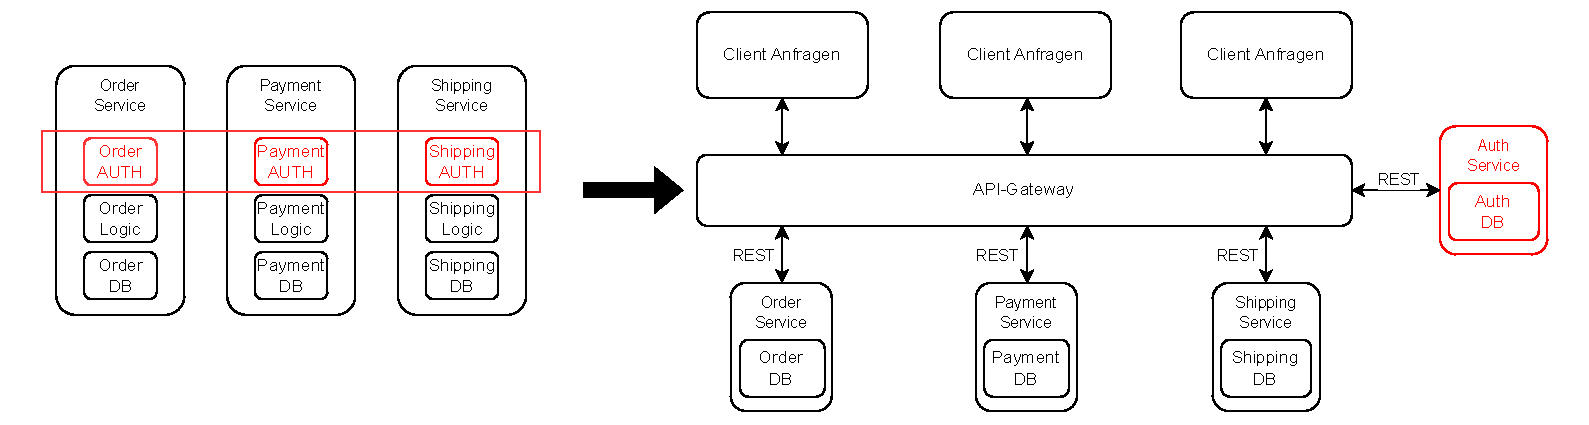
\includegraphics[width=0.5\textwidth]{images/layered/ecommerce-example}
    \caption{Layered Microservice Architecture: Beispiel E-Commerce}
    \label{fig:layered}
\end{figure}

Mit der Einführung einer zentralen Authentifizierungsschicht kann die Authentifizierungslogik
an einer einzigen Stelle gebündelt und bei Bedarf angepasst werden, ohne Änderungen in den
einzelnen Services vornehmen zu müssen.
Dies bietet insbesondere in Unternehmen mit einer Vielzahl von Services signifikante Zeit- und Kosteneinsparungen.

Ein weiterer Vorteil besteht darin, dass die Authentifizierung für sämtliche Dienste
zentral über ein API-Gateway durchgeführt wird, wodurch eine wiederholte Authentifizierung
auf Service-Ebene entfällt.
Diese Entlastung erlaubt es den einzelnen Services, sich ausschließlich auf ihre
Kernfunktionalität zu konzentrieren, während die Authentifizierung ausgelagert ist.

Die vollständige Implementierung des E-Commerce-Beispiels ist bei GitHub \footnote{https://github.com/Beleg-6-EAP/demo-microservice-ecommerce} zu finden.

Die klare Trennung der Verantwortlichkeiten fördert die Zusammenarbeit in kleinen, autonomen
Teams, da jedes Team unabhängig an einer Schicht arbeiten kann.
Zudem ermöglicht das Prinzip der Isolation der Schichten eine höhere Flexibilität gegenüber wechselnden Anforderungen.
Durch die Wiederverwendbarkeit in der Layered Architecture wird Mehraufwand vermieden und duplizierter
Code reduziert, was zu kürzeren Iterationen und häufigeren Auslieferungen führt.

Das Beispiel verdeutlicht zudem, dass die Layered Architecture sich hervorragend mit agilen
Architekturen wie Microservices kombinieren lässt.
Diese Synergie trägt entscheidend dazu bei, die Agilität des Systems nachhaltig zu steigern.
\section{Moderne Enterprise-Architekturen}

\subsection{Event-Driven Architecture}
Die Event-Driven Architecture wählt als Basis einen anderen Ausgangspunkt als die bisherigen Architekturmuster.
Während bei letzteren Komponenten Dienste bereitstellen, welche von anderen Komponenten explizit genutzt werden,
verhalten sich Dienst-bereitstellende Komponenten in der Event-Driven Architecture reaktiv,
werden also implizit von Dienst-konsumierenden Komponenten genutzt \cite{garlanShawImplizit}.
Ein System reagiert somit asynchron auf Zustandsänderungen, also Ereignisse in diesem System \cite{eda}.
Die in dieser Architektur minimalen Einheiten, welche Informationen einer Zustandsänderung kapseln, werden \textit{Events} genannt.
Die Idee der impliziten Behandlung von Ereignissen ist nicht neu und taucht erstmals 1994 im von Garlan und Shaw publizierten Papier
\textit{\enquote{An introduction to Software Architecture}} auf.

Betrachten wir im Folgenden die Basis-Bestandteile der Event-Driven Architecture:
\begin{itemize}
  \item Ereignis (englisch \textit{Event}): Kapselt Information einer Zustandsänderung eines Systems
  \item Produzent (englisch \textit{Producer}): Komponente, die Event erzeugt
  \item Herausgeber (englisch \textit{Publisher}): Komponente, die, von Produzenten erzeugte, Events publiziert
  \item Konsument (englisch \textit{Consumer}): Reagiert auf publizierte Events
  \item Vermittler (englisch \textit{Mediator}): Liegt zwischen Produzenten und Konsumenten - filtert Events und verteilt diese auf Konsumenten
  \item Event-Bus: Oft auch \textit{Event-Broker} genannt - bietet die Infrastruktur für die Gesamtheit der Vermittler
\end{itemize}
Abstrakt kann ein Event als ein Vertrag zwischen Produzenten und Konsumenten am Event-Bus betrachtet werden.
Der Konsument nutzt die Spezifikation des Events am Bus, der Produzent implementiert jene Spezifikation.
Abbildung \ref{fig:eda} stellt diesen Vertrag dar.

\begin{figure}[!h]
  \centering
  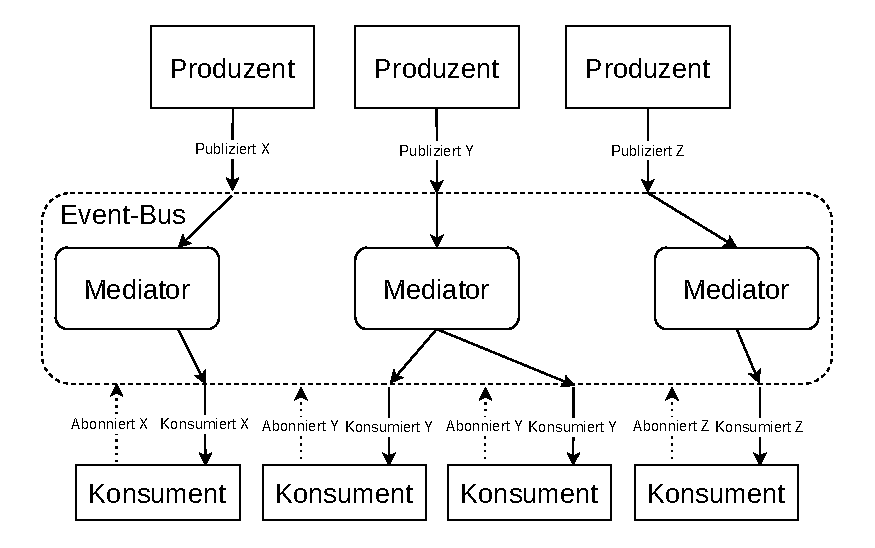
\includegraphics[width=\linewidth]{images/eda/eda.drawio}
  \caption{Vertrag zwischen Produzenten und Konsumenten am Event-Bus}
  \label{fig:eda}
\end{figure}

Durch den Vertrag weisen die Events am Event-Bus starke Kohäsion und somit lose Kopplung auf.
Diese lose Kopplung minimiert nicht nur kaskadierende Fehler, sondern ermöglicht agilen Entwickler-Teams durch klar abgegrenzte Features einfach definierbare Iterationen
- eine Menge von Events, deren Erzeugung und Konsumierung.

Weiter sind Events oft nah an dem, was Ereignisse in realen Prozessen sind, also domain-driven.
Gebündelt ermöglichen obige Punkte die kontinuierliche Auslieferung von Software in kurzen Intervallen.

Außerdem garantiert die asynchrone Behandlung von Ereignissen zusammen mit der loosen Kopplung maximale Skalierung.
Daher sind Event-Driven Architekturen besonders für datenintensive Echtzeit-Anwendungen wie IoT (Internet of Things) und Analytics geeignet \cite{iotEda}.

Die Agilität der Architektur kann weiter erhöht werden, indem der event-basierte Aspekt mit weiteren agilen Strukturen wie Microservices oder cloud-nativen Serverless-Functions kombiniert wird.
Die damit einhergehende Komplexität stellt teilweise hohe Anforderungen an die Entwickler.
Aufgrund der Asynchronität der Behandlung von Ereignissen ist die Testung des Systems meist schwer und die Fehlerbehandlung essentiell.
Mögliche Problemquellen schließen dabei unter anderem Event-Verlust, erhöhte Latenz und Inkonsistenz ein.
Die hohen Anforderungen an die Entwickler verlangen viel Vertrauen in jene, einer der zentralen Punkte des agilen Manifests \cite{agileManifesto}.
Insgesamt weist die Event-Driven Architecture also eine sehr hohe Agilität auf und ist damit besonders für moderne Software und ihre stetig wechselnden Anforderungen geeignet.

% TODO: Jetzt bestenfalls übergreifendes Beispiel

\section{Fallstudien und Praxisbeispiele}
Blah \ldots

\section{Diskussion}

\section{Zusammenfassung und Ausblick}
%(Überblick über die gesamte Arbeit, Rückführung auf Aussagen aus Kapitel 1 durchführen, offene Punkte als neue Forschungsfragen definieren)






\bibliographystyle{ACM-Reference-Format}
\bibliography{main}

\appendix

\section{Anhang 1}

\subsection{Übungsaufgaben}
Blah \ldots

\section{Anhang 2}
Blah \ldots

\end{document}
\endinput
